\documentclass[../thesis.tex]{subfiles}
\begin{document}

\chapter{Simulation model}
\label{chp:model}

Within this part the creation process of the simulation model will be explained in greater detail. At first the three basic equations the software solves will be given followed by a brief overview of the steps taken to create the model. Then the model's results are explained and compared to already done experiments for validation.

\section{model setup}
\label{sec:mod_setup}

In this section the steps needed to create the model within \texttt{ANSYS FLUENT} are explained.

\subsection{geometry creation}
The first of the model creation in \texttt{ANSYS FLUENT} is the modeling of the system's geometry. This geometry can either be created using the tools \texttt{ANSYS FLUENT} provides it self or be imported from an already existing CAD model. Within this work the geometry is created using ANSYS DesignModeler. In \autoref{fig:ansys_geometry} the designed model is shown and the used dimensions are listed in \autoref{tab:ansys_design}.

\begin{figure}[htbp]
	\centering
	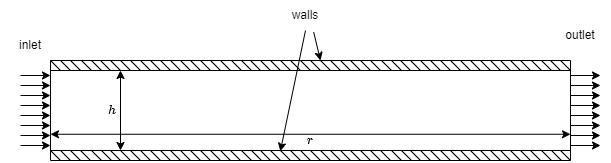
\includegraphics[width=\textwidth]{geometry}
	\caption{model geometry}
	\label{fig:ansys_geometry}
\end{figure}

\begin{table} [htb]
	\centering
	\caption{example model geometry dimensions}
	\begin{tabular}{ ccc }
		\hline
		variable & value & unit \\
		\hline
		$r$ & 30.0 & mm \\
		$h$ & 0.6 & mm \\
		\hline
		\label{tab:ansys_design}
	\end{tabular}
\end{table}

$h$ represents the height of the Hele-Shaw cell and $r$ is the radius of the cell. A value of 30mm is chosen here to reduce the amount of computational effort instead of modeling the hole cell with it's 50mm radius.

\subsection{meshing}

The next step in model design following the procedure shown in \autoref{fig:cdf_procedure} in \autoref{chp:theory} is meshing. An example of the generated mesh can be seen in \autoref{fig:ansys_meshing}.
\begin{figure}[htb]
	\centering
	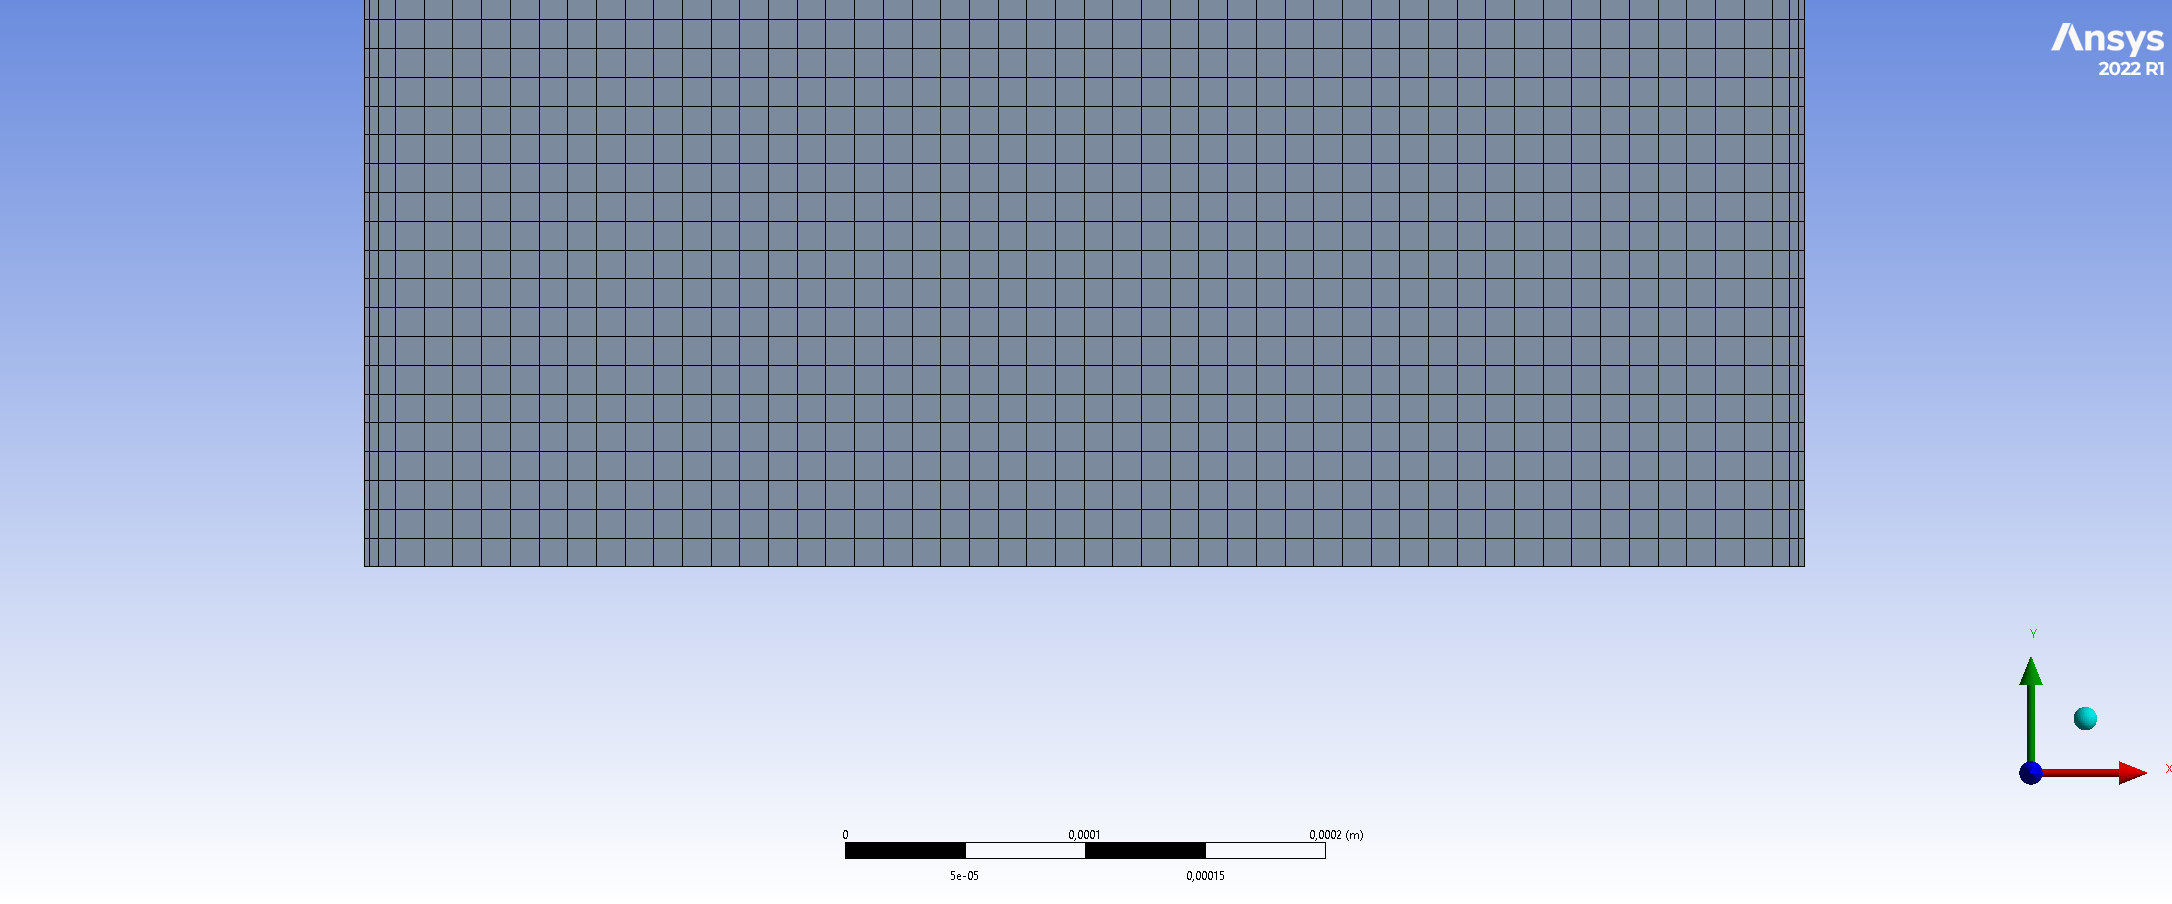
\includegraphics[scale=0.25]{Mesh}
	\caption{Ansys Meshing example}
	\label{fig:ansys_meshing}
\end{figure}
The figure shows the reactor's inlet section. The goal in meshing was to create rectangular grid out of squares or rectangles. Near the walls, that begin on the left and right side of the inlet, the mesh resolution is increased using two inflation layers. That is done to resolve the boundary layer of the flow near the walls. Having a mesh consisting mostly out of squares and rectangles is advantageous because the algorithm only stores the values at the cell's centre as mentioned in \autoref{sec:QUICK}. Having a mesh that can be seen as a 2 dimensional array makes post-processing a lot easier. How the results are extracted from the model's output will be explained in \autoref{sec: model res} in greater detail.

\subsection{solver settings}
\label{sec: setup}

To setup the model at first a few basic configuration steps need to done. The Settings that need to be applied are listed in \autoref{tab:ansys_setup_general}.

\begin{table} [htb]
	\centering
	\caption{General settings}
	\begin{tabular}{ ccc }
		\hline
		Section & Setting & value \\
		\hline
		Solver & Type & Pressure-Based \\
		Solver & Velocity Formulation & Absolute  \\
		Solver & Time &  Transient  \\
		Solver & 2D Space & Axisymmetric \\
		\hline
		\label{tab:ansys_setup_general}
	\end{tabular}
\end{table}
With these general settings are done the used models need to be activated. The used models settings are given in \autoref{tab:ansys_setup_models}.

\begin{table} [htb]
	\centering
	\caption{model settings}
	\begin{tabular}{ cc }
		\hline
		variable & value \\
		\hline
		Energy & On \\
		Viscous & Laminar \\
		Species & (Species Transport, Reactions)  \\
		\hline
		\label{tab:ansys_setup_models}
	\end{tabular}
\end{table}

After the correct models are turned on and parametrized the species taking part within the model are defined. Within this case 4 fluids are needed. The example configuration of one of the fluids taking part within the reaction is shown in \autoref{tab:ansys_setup_materials}. The table shows the configuration of one of the educts.
\begin{table} [htb]
	\centering
	\caption{Example fluid settings}
	\begin{tabular}{ ccc }
		\hline
		variable & value & unit \\
		\hline
		\\[-1em]
		$\rho$ & 1000 & $\frac{\text{kg}}{\text{m³}}$ \\
		\\[-1em]
		$\nu$ & 0.001003 & $\frac{\text{m²}}{s}$ \\
		\\[-1em]
		$M$ & 100 & $\frac{\text{g}}{\text{mol}}$ \\
		\\[-1em]
		$D$ & 8.22e-10 & $\frac{\text{m²}}{s}$\\
		\\[-1em]
		\hline
		\label{tab:ansys_setup_materials}
	\end{tabular}
\end{table}
All other values, namely enthalpies and other thermodynamic properties are the same for all the fluids and equal to the values of water. Since 3 fluids take part in the reaction and 4 fluids are needed to setup the model the yet missing fluid is water. It is needed to be able to set a molar concentration at the inlet that is lower than the maximum of 1. After this the values from the fluids should be carried over to the mixture configuration within the new existing Mixture tab. With the mixture settings the reaction parameters are set. The parameters set for the reaction are stated in \autoref{tab:ansys_setup_rection}.
\begin{table} [htb]
	\centering
	\caption{reaction settings}
	\begin{tabular}{ ccc }
		\hline
		variable & value & unit \\
		\hline
		Reaction Type & Volumetric & - \\
		Stoich. Coefficient fluid\_a & 1 & - \\
		Stoich. Coefficient fluid\_b & 1 & - \\
		Stoich. Coefficient fluid\_c & 1 & - \\
		Rate Exponent fluid\_a & 1 & - \\
		Rate Exponent fluid\_b & 1 & - \\
		Rate Exponent fluid\_c & 0 & - \\
		Pre-Exponential Factor & 1e15 & - \\
		\\[-1em]
		Activation Energy & 1e4 & $\frac{\text{J}}{\text{mol}}$ \\
		\\[-1em]
		\hline
		\label{tab:ansys_setup_rection}
	\end{tabular}
\end{table}
To achieve a nearly instant reaction when molecules of the two species A and B meet the rate constant which also known as Pre-Exponential Factor (see \autoref{eqn:reaction}) is set to a very high value. The Activation Energy is set to a value that the given temperature is high enough to let the reaction happen.

After the reaction is setup correctly the boundary conditions are being set. Conditions need to be set for the inlet, outlet and the walls. All information needed to configure the boundary conditions are visible in \autoref{tab:ansys_setup_boundary}

\begin{table} [htb]
	\centering
	\caption{boundary conditions}
	\begin{tabular}{ cccc }
		\hline
		place & variable & value & unit \\
		\hline
		inlet & Type & velocity-inlet & - \\
		inlet & Velocity Specification Method & Magnitude, Normal to Boundary & - \\
		\\[-1em]
		inlet & Velocity Magnitude & e.g. 4e-3 & $\frac{\text{m}}{\text{s}}$ \\
		\\[-1em]
		inlet & Temperature & 300 & K \\
		inlet & fluid\_a & 5.4e-4 & - \\
		outlet & Type & pressure-outlet & - \\
		outlet & Gauge Pressure & 20 & Pa \\
		outlet & Prevent Reverse Flow & yes & - \\
		wall & Type & wall & - \\
		wall & Wall Motion & Stationary Wall & - \\
		wall & Shear Condition & No Slip & - \\
		\hline
		\label{tab:ansys_setup_boundary}
	\end{tabular}
\end{table}
There is a homogenous velocity profile set at the inlet normal to the boundary. At the inlet the amount of $fluid\_a$ has to set as a mole fraction as well. To get matching conditions to the already performed experiments the mole fraction needs to be calculated from a given concentration. Assuming the values from \autoref{tab:ansys_setup_molefrac} are known the mole fraction can be calculated using \autoref{eqn:molefrac}.

\begin{table} [htb]
	\centering
	\caption{needed variables for mole and mass fraction calculation}
	\begin{tabular}{ cccc }
		\hline
		variable & description & value & unit \\
		\hline
		$M_{W}$ & Molar Mass water & 18 & g/mol \\
		$M_{A}$ & Molar Mass $fluid\_a$ & 100 & g/mol \\
		$M_{fluid\_b}$ & Molar Mass $fluid\_b$ & 100 & g/mol \\
		$\rho_{water}$ & Density water & 1000 & kg/m³ \\
		$c_{fluid\_b}$ & Concentration $fluid\_b$ & 0.03 & mol/l \\
		$c_{water}$ & Concentration water & 55.55 & mol/l \\
		$Q$ & inlet flow rate &  e.g. 0.144 & ml/min \\
		\hline
		\label{tab:ansys_setup_molefrac}
	\end{tabular}
\end{table}

\begin{equation}
	\label{eqn:molefrac}
	x_{B} =\dfrac{\dot{n_{B}}}{\dot{n_{B}} + \dot{n_{W}}} = \dfrac{c_{B} \cdot Q}{c_{B} \cdot Q + c_{W} \cdot Q} = \dfrac{c_{B}}{c_{B} + c_{W}} \approx 0 \text{.}00054
\end{equation}
Since the concentration for $fluid\_{A}$ within the internal domain has to be setup as mass fraction the needed value can be calculated using \autoref{eqn:massfrac}.

\begin{equation}
	\label{eqn:massfrac}
	\varphi_{A} =\dfrac{n_{A} \cdot M_{A}}{n_{A} \cdot M_{A} + n_{W} \cdot M_{W}} = \dfrac{c_{A} \cdot M_{A}}{c_{A} \cdot M_{A} + c_{W} \cdot M_{W}} \approx \text{0.003}
\end{equation}

The temperature is set to 300 K at the inlet and within the hole internal domain. The outlet is configured to be a pressure outlet without reverse flow to get physical valid results. At the walls the usual conditions applied to walls are set with no slip and stationary.

The next step performed is to setup the solution methods as shown in \autoref{tab:ansys_setup_sol_methods}. As the solving scheme the PISO algorithm is used, that is explained in \autoref{sec:sol_method}. For spatial discretization second order methods, as explained in \autoref{sec:QUICK}, are used. 
\begin{table} [htb]
	\centering
	\caption{solution methods}
	\begin{tabular}{ ccc }
		\hline
		tab & setting & method \\
		\hline
		Pressure-Velocity Coupling & Scheme & PISO \\
		Spatial Discretization & Pressure & Second Order \\
		Spatial Discretization & Momentum & QUICK \\
		Spatial Discretization & $fluid\_a$ & Second Order Upwind \\
		Spatial Discretization & $fluid\_b$ & Second Order Upwind \\
		Spatial Discretization & $fluid\_c$ & Second Order Upwind \\
		Spatial Discretization & Energy & Second Order Upwind \\
		\hline		
		\label{tab:ansys_setup_sol_methods}
	\end{tabular}
\end{table}

As a last step in the model creation procedure the time settings need to be set. An adaptive method is chosen which is based on the CFL-Number $c$. This number can be calculated using \autoref{eqn:cfl} and is also known as Courant-Number. It is influenced by the velocity $u$, the time step $ \Delta t$ and the spacial discretization $\Delta x$. It is best practice to keep this number below or equal to 1 for stability reasons. This can be otherwise thought of as a limiting factor in a way that to rapid changes from one cell to the next one between time steps are inhibited.  
\begin{equation}
	\label{eqn:cfl}
	c = \dfrac{u \cdot \Delta t}{\Delta x}
\end{equation}
In this model the Courant-Number is set to 1 and the initial time step size is set to 0.01 seconds to get a compromise between simulation stability and calculation time. The time step size is updated after every calculation. The factor for time step changes are limited to 0.5 on the lower and 2 at the upper end. The time step algorithm decides for a time step change based on the Courant-Number. In addition to the model's time settings the interval the results are exported at need to be set. This in addition to the exported variables of interest can be set under $\texttt{Solution} \rightarrow \texttt{Activities} \rightarrow \texttt{Manage...}$.

\begin{table} [htb]
	\centering
	\caption{time settings}
	\begin{tabular}{ ccc }
		\hline
		variable & value & unit \\
		\hline
		Type & Adaptive & - \\
		Method & CFL-Based & - \\
		Duration Specification Method & Total Time & -\\
		Total Time & e.g. 20 & s \\
		Courant Number & 1 & - \\
		Fixed Timsteps & 1 & - \\
		Initial Time Step Size & 0.01 & s \\
		Max Iteration/Time Step & 30 & - \\
		Time Step Size Update Interval & 1 & - \\
		Minimum Time Step Size & e.g. 0.001 & s \\
		Maximum Time Step Size & e.g. 0.5 & s \\
		Minimum Step Change Factor & 0.5 & - \\
		Maximum Step Change Factor & 2 & - \\		
		\hline
		\label{tab:ansys_setup_time}
	\end{tabular}
\end{table}

\subsection{model evolution and refinement}
\label{sec: mod_evol}

Here the steps taken to receive the final model for each case are explained.

For each of the three different reactor geometries two to three meshes are created that are shown in \autoref{tab: reactor meshes}.

\begin{table} [htb]
	\centering
	\caption{case meshes}
	\begin{tabular}{ ccc }
		\hline
		reactor height [mm] & element size [m] & mesh elements \\
		\hline
		0.2 & 6e-6 & 185000\\
		0.2 & 4e-6 & 405000\\
		0.2 & 2e-6 & 1560000\\
		0.4 & 12e-6 & 92500\\
		0.4 & 8e-6 & 202500\\
		0.4 & 4e-6 & 780000\\
		0.6 & 4e-6 & 1155154\\
		0.6 & 2e-6 & 4560304\\
		\hline		
		\label{tab: reactor meshes}
	\end{tabular}
\end{table}

Each case is run for the coarsest mesh and the results are inspected. If the Courant-Number field does not show values larger than 1 and the velocity field looks believable too the run is called successful. If that is not the case the next finer mesh is chosen and the case is run again.

For the Peclet-Number 3 different values are chosen and for the Schmidt number 2 values are implemented. These values are in case of $Pe$ 500, 931 and 2050. The Schmidt number $Sc$ has either a value of 2430 or 12000. The Schmidt number mostly influences the diffusion coefficient as the viscosity $\nu$ does not change a lot between the two chosen values. Having fixed the Schmidt number and the diffusion coefficient, the Peclet-Number mostly influences the input velocity. An overview of the performed cases and their input variable values can be seen in \autoref{tab: cases}. Besides the reactor height $h$, the Peclet-Number $Pe$ and other needed input variables, the simulation time and export time in seconds need to be set. The simulation time is the physical time that represents for how long the model should be simulated. The export time sets the time interval in seconds at which results are exported during the transient simulation. These results, that contain all the values for all variables of interest for each cell, are the basis for further analysis. How the results are obtained and how they are further processed is explained in \autoref{sec: model res}.

\begin{landscape}
	\begin{table}[htb]
		\centering
		\caption{simulation cases}
		\label{tab: cases}
		\small
		\begin{tabular}{cccccccccc}
			\textbf{h [m]} & \textbf{Pe} & \textbf{Sc} & \textbf{$\nu$ [m²/s]} & \textbf{$D$ [m²/s]} & \textbf{u [m/s]} & \textbf{$x_A$} & \textbf{$\varphi_B$} & \textbf{simulation time [s]} & \textbf{export time [s]} \\
			\hline
			2.00E-04            & 500         & 2430        & 1.00E-06               & 4.11E-10               & 1.03E-03              & 5.40E-04      & 3.00E-03        & 60                            & 0.5                       \\
			2.00E-04            & 500         & 12000       & 1.20E-06               & 1.00E-10               & 2.50E-04              & 5.40E-04      & 3.00E-03        & 60                            & 0.1                       \\
			2.00E-04            & 500         & 120000      & 1.20E-06               & 1.00E-11               & 2.50E-05              & 5.40E-04      & 3.00E-03        & 60                            & 0.1                       \\
			2.00E-04            & 931         & 2430        & 1.00E-06               & 4.11E-10               & 1.91E-03              & 5.40E-04      & 3.00E-03        & 60                            & 0.5                       \\
			2.00E-04            & 931         & 12000       & 1.20E-06               & 1.00E-10               & 4.66E-04              & 5.40E-04      & 3.00E-03        & 60                            & 0.1                       \\
			2.00E-04            & 931         & 120000      & 1.20E-06               & 1.00E-11               & 4.66E-05              & 5.40E-04      & 3.00E-03        & 60                            & 0.1                       \\
			2.00E-04            & 2050        & 2430        & 1.00E-06               & 4.11E-10               & 4.21E-03              & 5.40E-04      & 3.00E-03        & 60                            & 0.5                       \\
			2.00E-04            & 2050        & 12000       & 1.20E-06               & 1.00E-10               & 1.02E-03              & 5.40E-04      & 3.00E-03        & 60                            & 0.1                       \\
			2.00E-04            & 2050        & 120000      & 1.20E-06               & 1.00E-11               & 1.02E-04              & 5.40E-04      & 3.00E-03        & 60                            & 0.1                       \\
			4.00E-04            & 500         & 2430        & 1.00E-06               & 4.11E-10               & 5.14E-04              & 5.40E-04      & 3.00E-03        & 60                            & 0.5                       \\
			4.00E-04            & 500         & 12000       & 1.20E-06               & 1.00E-10               & 1.25E-04              & 5.40E-04      & 3.00E-03        & 60                            & 0.1                       \\
			4.00E-04            & 500         & 120000      & 1.20E-06               & 1.00E-11               & 1.25E-05              & 5.40E-04      & 3.00E-03        & 60                            & 0.1                       \\
			4.00E-04            & 931         & 12000       & 1.20E-06               & 1.00E-10               & 2.33E-04              & 5.40E-04      & 3.00E-03        & 60                            & 0.1                       \\
			4.00E-04            & 931         & 2430        & 1.00E-06               & 4.11E-10               & 9.57E-04              & 5.40E-04      & 3.00E-03        & 60                            & 0.5                       \\
			4.00E-04            & 931         & 120000      & 1.20E-06               & 1.00E-11               & 2.33E-05              & 5.40E-04      & 3.00E-03        & 60                            & 0.1                       \\
			4.00E-04            & 2050        & 12000       & 1.20E-06               & 1.00E-10               & 5.12E-04              & 5.40E-04      & 3.00E-03        & 60                            & 0.5                       \\
			4.00E-04            & 2050        & 2430        & 1.00E-06               & 4.11E-10               & 2.10E-03              & 5.40E-04      & 3.00E-03        & 60                            & 0.5                       \\
			4.00E-04            & 2050        & 120000      & 1.20E-06               & 1.00E-11               & 5.12E-05              & 5.40E-04      & 3.00E-03        & 60                            & 0.1                       \\
			6.00E-04            & 500         & 2430        & 1.00E-06               & 4.11E-10               & 3.43E-04              & 5.40E-04      & 3.00E-03        & 60                            & 0.5                       \\
			6.00E-04            & 500         & 12000       & 1.20E-06               & 1.00E-10               & 8.33E-05              & 5.40E-04      & 3.00E-03        & 60                            & 0.5                       \\
			6.00E-04            & 500         & 120000      & 1.20E-06               & 1.00E-11               & 8.33E-06              & 5.40E-04      & 3.00E-03        & 60                            & 0.5                       \\
			6.00E-04            & 931         & 12000       & 1.20E-06               & 1.00E-10               & 1.55E-04              & 5.40E-04      & 3.00E-03        & 60                            & 0.5                       \\
			6.00E-04            & 931         & 2430        & 1.00E-06               & 4.11E-10               & 6.38E-04              & 5.40E-04      & 3.00E-03        & 60                            & 0.5                       \\
			6.00E-04            & 931         & 120000      & 1.20E-06               & 1.00E-11               & 1.55E-05              & 5.40E-04      & 3.00E-03        & 60                            & 0.5                       \\
			6.00E-04            & 2050        & 12000       & 1.20E-06               & 1.00E-10               & 3.41E-05              & 5.40E-04      & 3.00E-03        & 60                            & 0.5                       \\
			6.00E-04            & 2050        & 2430        & 1.00E-06               & 4.11E-10               & 1.40E-03              & 5.40E-04      & 3.00E-03        & 60                            & 0.5                       \\
			6.00E-04            & 2050        & 120000      & 1.20E-06               & 1.00E-11               & 3.41E-05              & 5.40E-04      & 3.00E-03        & 60                            & 0.5						\\
			\hline      
		\end{tabular}
	\end{table}
\end{landscape}

    

\end{document}